\documentclass[border=4pt]{standalone}
% Shared style for every diagram. Colour-blind-safe palette (Okabe-Ito).
\usepackage[T1]{fontenc}
\usepackage{helvet}
\renewcommand{\familydefault}{\sfdefault}
\usepackage{tikz}
\usetikzlibrary{arrows.meta,positioning,fit,backgrounds,calc,shapes.geometric,decorations.pathreplacing}
\definecolor{cblue}{HTML}{0072B2}
\definecolor{corange}{HTML}{E69F00}
\definecolor{cgreen}{HTML}{009E73}
\definecolor{cred}{HTML}{D55E00}
\definecolor{cpurple}{HTML}{CC79A7}
\definecolor{cgrey}{HTML}{6B7280}
\definecolor{csky}{HTML}{56B4E9}
\tikzset{
  >={Stealth[length=2.2mm]},
  box/.style={draw, rounded corners=3pt, align=center, minimum height=11mm, minimum width=22mm, font=\small, line width=0.7pt},
  real/.style={box, draw=cblue, fill=cblue!8},
  sim/.style={box, draw=corange, fill=corange!12},
  future/.style={box, draw=cgrey, dashed, fill=white},
  flow/.style={->, line width=0.8pt, draw=black!75},
  dflow/.style={->, line width=0.8pt, dashed, draw=cgrey},
  lbl/.style={font=\scriptsize, text=black!70},
  group/.style={draw=black!25, rounded corners=6pt, inner sep=6pt},
}

\begin{document}
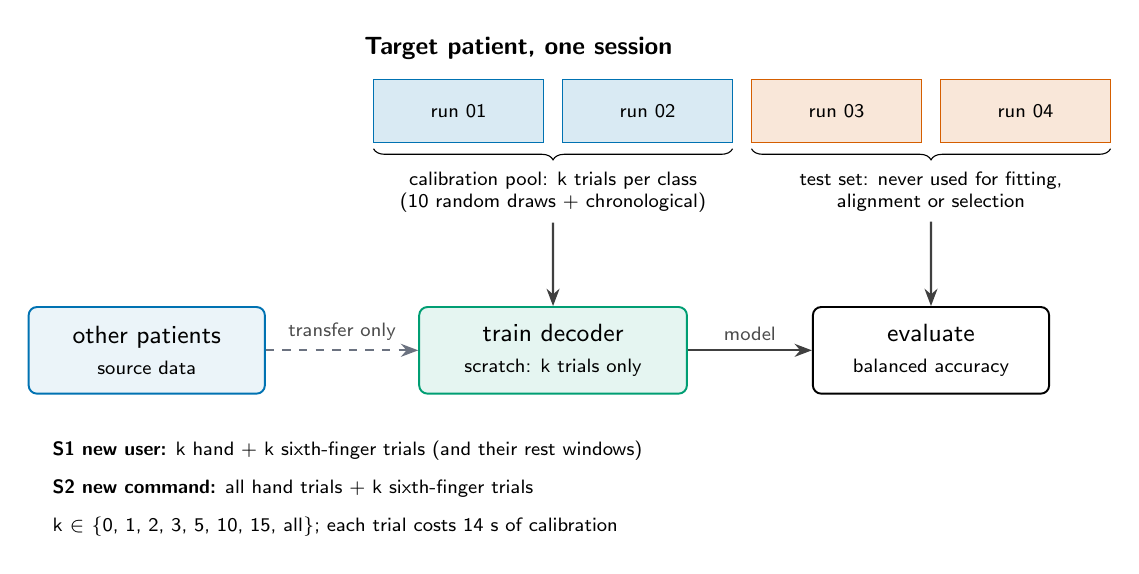
\begin{tikzpicture}[x=12mm, y=8mm]
  \node[font=\small\bfseries, anchor=west] at (-0.2,3.1) {Target patient, one session};
  \foreach \r/\c/\t in {0/cblue/run 01, 1/cblue/run 02, 2/cred/run 03, 3/cred/run 04} {
    \draw[fill=\c!15, draw=\c] (\r*2,1.6) rectangle (\r*2+1.8,2.6);
    \node[font=\scriptsize] at (\r*2+0.9,2.1) {\t};
  }
  \draw[decorate, decoration={brace, amplitude=4pt, mirror}] (0,1.5) -- (3.8,1.5) node[midway, below=5pt, font=\scriptsize, align=center] (pool) {calibration pool: k trials per class\\(10 random draws + chronological)};
  \draw[decorate, decoration={brace, amplitude=4pt, mirror}] (4,1.5) -- (7.8,1.5) node[midway, below=5pt, font=\scriptsize, align=center] (test) {test set: never used for fitting,\\alignment or selection};
  \node[real, minimum width=30mm] (src) at (-2.4,-1.7) {other patients\\\scriptsize source data};
  \node[box, minimum width=34mm, draw=cgreen, fill=cgreen!10] (train) at (1.9,-1.7) {train decoder\\\scriptsize scratch: k trials only};
  \node[box, minimum width=30mm] (eval) at (5.9,-1.7) {evaluate\\\scriptsize balanced accuracy};
  \draw[flow] (pool.south) -- (train.north);
  \draw[dflow] (src) -- node[lbl, above] {transfer only} (train);
  \draw[flow] (train) -- node[lbl, above] {model} (eval);
  \draw[flow] (test.south) -- (eval.north);
  \node[font=\scriptsize, anchor=west, align=left] at (-3.5,-3.3) {\textbf{S1 new user:} k hand + k sixth-finger trials (and their rest windows)};
  \node[font=\scriptsize, anchor=west, align=left] at (-3.5,-3.9) {\textbf{S2 new command:} all hand trials + k sixth-finger trials};
  \node[font=\scriptsize, anchor=west, align=left] at (-3.5,-4.5) {k $\in$ \{0, 1, 2, 3, 5, 10, 15, all\};\ each trial costs 14 s of calibration};
\end{tikzpicture}
\end{document}
